\noindent \texttt{V: 25-10-2022 17:28:00}
\section*{Experimento: - CAPACITÂNCIA}
	\section{Objetivos}
	
	Estudar o efeito capacitivo entre as placas de um capacitor variável de placas paralelas - Figura \ref{fig:cidepe-capacitor}, verificando a relação da capacitância $C=\epsilon_{0} A/d$ em função da distância $d$ entre as placas; Medir a constante de permissividade ${\epsilon}_{0}$ e medir a constante dielétrica de distintos materiais isolantes como papel, \href{https://pt.wikipedia.org/wiki/Espuma_vin\%C3\%ADlica_acetinada}{ E.V.A (\textit{Ethylene Vinyl Acetate})} e isopor.	
	\section{Material utilizado}
	
\begin{wrapfigure}{r}{0.7\textwidth}
    \centering
    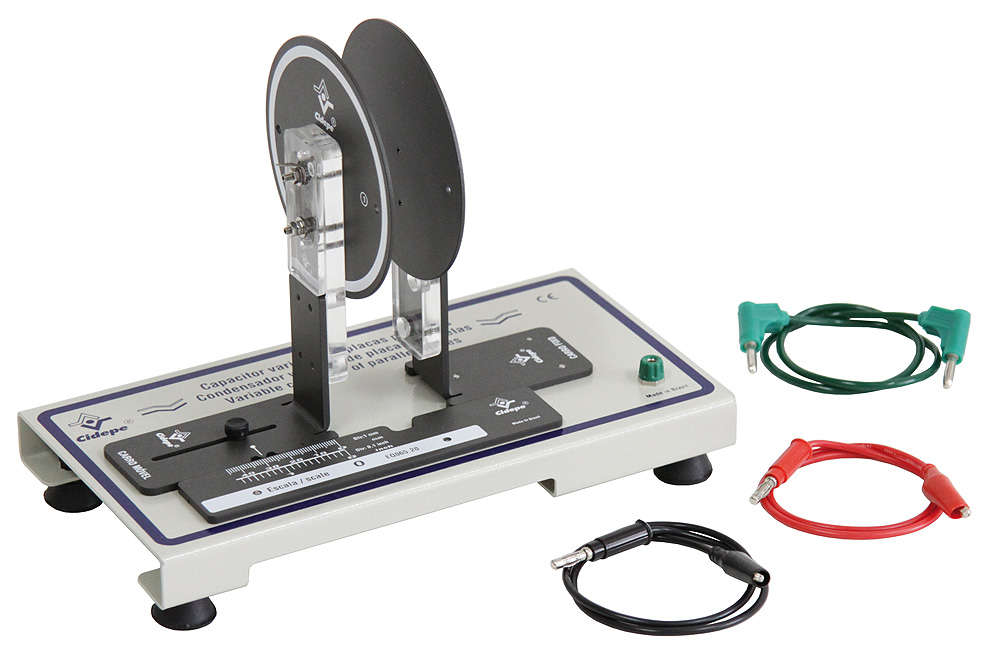
\includegraphics[width=.36\textwidth]{img/cidepe-capacitor.jpg}
    \caption{Capacitor de placas paralelas com separação variável montado em isolante acrílico. \textit{Fonte: Cidepe}.}
    \label{fig:cidepe-capacitor}
\end{wrapfigure}
	
	\begin{itemize}
		\item[a)] Um capacitor variável de placas paralelas: 2,3 pF - 280 pF;
		\item[b)] Um medidor digital de capacitância;
		\item[c)] Dois fios ou cabos condutores;
		\item[d)] Um papel milimetrado;
		\item[e)] Folhas de papel ou papelão;
		\item[f)] Lâminas de isolantes E.V.A, EPS (Isopor), Vidro, Acrílico,etc;
		\item[j)] Uma régua ou trena ou paquímetro.
		
	\end{itemize}
	
\begin{comment}
\begin{figure}[H]
	\centering
	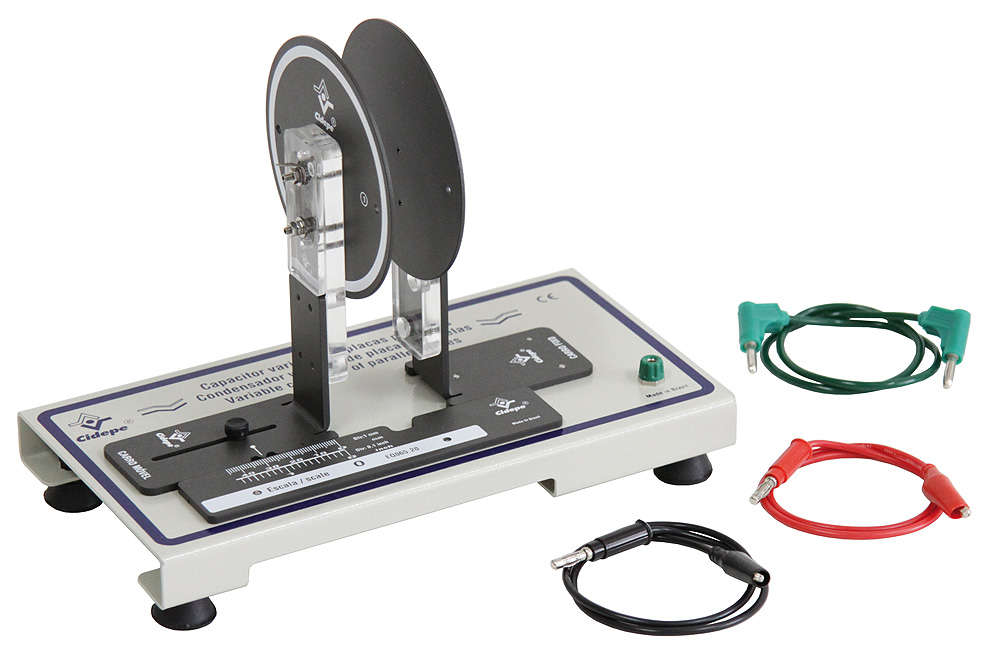
\includegraphics[scale=.3]{img/cidepe-capacitor.jpg}
	\caption{Capacitor de placas paralelas com separação variável montado em isolante acrílico. Fonte: Cidepe.}
	\label{fig:imagem1}
\end{figure}
\end{comment}


\section{Fundamentos teóricos}
	
	Se preenchermos o espaço entre as placas de um capacitor com um dielétrico (isolante), o que acontecerá com a capacitância? \textbf{Michel Faraday} (1791-1867) investigou este assunto pela primeira vez em 1837. Usando equipamento simples, ele descobriu que a capacitância aumentava por um fator $\kappa$, que ele chamou de constante dielétrica do material isolante. Outro efeito importante na introdução do dielétrico no capacitor é limitar a diferença de potencial que se pode aplicar entre as placas a um certo valor ${V}_{max}$, chamado de potencial de ruptura. Se este valor for excedido, o material dielétrico se romperá e formará um caminho condutor ({\color{red}\textbf{arco elétrico}}) entre as placas. Logo, todo material dielétrico possui uma rigidez dielétrica característica, que é o valor máximo do campo elétrico que um isolante pode tolerar sem se romper e se tornar um condutor (para o ar a rigidez dielétrica é $~3\times10^{6} \,V.m^{-1}$, ou seja tensões ou diferenças de potencial ${V}_{max}$ acima desses valores, permitem a ocorrência de um \textbf{arco elétrico} ou popularmente \textit{raio/faísca/centelha}). Na Tabela \ref{tab:rigidez-materiais} são mostradas algumas constantes dielétricas importantes.
	
	%tabela 1
	\begin{table}[H]
		\centering
	\begin{tabular}{l|c|c}
		\hline 
		Material & Constante Dielétrica, $\kappa$ & Rigidez Dielétrica $E_{max} (10^{6}\,V.m^{-1})$ \\ 
		\hline 
		Ar(1 atm) & 1,0006 & 3 \\ 
        Madeira & & 10 \\
        Borracha & & 12 \\
	Papel & 3,5 & 16 \\ 
        Poliéster & 3,6 & 21,7 \\ 
        Vidro & & 30 \\
        Mica & & 60 \\
        Teflon & & 80 \\
        
		\hline 
	\end{tabular} 
		\caption{Constante dielétrica e rigidez dielétrica}
		\label{tab:rigidez-materiais}
	\end{table}

	\section{Procedimento experimental}
	
	\subsection{A - MEDIDA DA PERMISSIVIDADE ELÉTRICA ($\epsilon_{0}$)}
	
	\begin{itemize}
		\item[a)] Certifique-se de que o capacitor esteja descarregado, fazendo contato entre as duas placas por meio de um fio ou cabo condutor;
		\item[b)] Meça o diâmetro, calcule o raio e com este a área das placas do capacitor (use: $A=\pi r^2$, onde $r$ é o \textbf{raio} das placas). Anote os resultados na Tabela \ref{tab:area-placas};
		
		%tabela 2
		\begin{table}[H]
			\centering
		\begin{tabular}{|c|c|}
			\hline 
			Diâmetro das Placas ($m$) & Área das Placas do Capacitor ($m^2$)\\ 
			\hline
			&  \\ 
			\hline 
		\end{tabular}
			\caption{\label{tab:area-placas} Diâmetro e área do capacitor}
		\end{table}
		
		\item[c)] Fazer a conexão do medidor de capacitância nas placas do capacitor. \textbf{Zerar o aparelho antes de fazer a medida};
		\item[d)] Com a chave seletora do medidor em 200 pF, estabeleça um espaçamento aproximado de 1,0 ou 10 mm entre as placas do capacitor. Anote o valor da capacitância $C_{exp}$ na Tabela \ref{tab:cte-dieletrica}; 
		\item[e)] Calcule a constante de permissividade (use a relação: $ \epsilon_{0}= C_{exp} \, d / A. \kappa_{ar} $). Anote o resultado na Tabela \ref{tab:cte-dieletrica};
		\item[f)] Calcule o erro experimental, entre o valor teórico (da literatura), e o valor experimental (medido). Anote o resultado na Tabela \ref{tab:cte-dieletrica}. 
	
		%tabela 3
		\begin{table}[H]
			\centering
		\begin{tabular}{|c|c|c|c|c|}
			\hline 
			$C_{exp}$ (pF) & $\epsilon_{0}$ (Teórico)(pF) & $\epsilon_{0}$ (experimental)(pF) & Erro (Absoluto) & Erro (\%)  \\ 
			\hline 
			& 8,85 & & & \\ 
			\hline 
		\end{tabular}
			\caption{Medição da constante dielétrica}
			\label{tab:cte-dieletrica}
		\end{table} 
	\end{itemize}
	
	\subsection{B - VARIAÇÃO DA CAPACITÂNCIA COM A SEPARAÇÃO ENTRE AS PLACAS}
	
	\begin{itemize}
		\item[a)] Certifique-se de que o capacitor esteja descarregado;
		\item[b)] Com a chave seletora do medidor em 200 pF, varie a distância entre as placas de 1 mm em 1 mm até 10 mm (5 mm em 5 mm até 50 mm no Capacitor \href{https://www.cidepe.com.br/index.php/br/produtos-interna/capacitor-variavel-de-placas-paralelas-e-cabos-0-a-255-pf-1875}{Cidepe EQ065D} ou similar). Para cada variação meça a capacitância correspondente ({\color{red}\textbf{Para uma melhor precisão, a partir da segunda medida selecione a posição da chave em $200 \,\mu F$}}). Anote os valores das capacitâncias $ C_{exp} $ na Tabela \ref{tab:c-versus-inv-d};

		%tabela 4
		\begin{table}[H]
			\centering
		\begin{tabu}{| l | X[c] | X[c] | X[c] | X[c] | X[c] | X[c] | X[c] | X[c] | X[c] | X[c] |}
			\hline 
			d ($mm$) &  &  &  &  &  &  &  &  &  &  \\ 
			\hline 
			$C_{exp} \,(pF$) &  &  &  &  &  &  &  &  &  &  \\ 
			\hline 
			1/d ($mm^{-1}$) &  &  &  &  &  &  &  &  &  &  \\ 
			\hline 
		\end{tabu} 
			\caption{Variação da capacitância em função de d e 1/d}
			\label{tab:c-versus-inv-d}
		\end{table} 
	
		\item[c)] Faça um gráfico, digital ou em papel milimetrado, de $ C_{exp} \times d $ e em seguida de $ C_{exp} \times (1/d) $;
		\item[d)] Obtenha o coeficiente angular \textbf{$\alpha$} da reta $ C_{exp} \times (1/d) $ e compare com o valor do produto $ \kappa_{ar} \epsilon_{0} A$. Anote os valores na Tabela \ref{tab:coeficientes}; 
		\item[e)] Calcule o erro experimental absoluto e percentual.
		
		%tabela 5
		\begin{table}[H]
			\centering
		\begin{tabular}{|c|c|c|c|}
			\hline 
			Coeficiente angular $\alpha$ (pF.m) & $\kappa_{ar} \epsilon_{0} A$ (Teórico)(pFm) & Erro (Absoluto) & Erro (\%) \\ 
			\hline 
			&  &  & \\ 
			\hline 
		\end{tabular}
			\caption{Coeficientes e constantes}
			\label{tab:coeficientes}
		\end{table} 
		
	\end{itemize}
	
	\subsection{C - MEDIDAS DAS CONSTANTES DIELÉTRICAS DOS ISOLANTES}
	
	\begin{itemize}
		\item[a)] Certifique-se de que o capacitor esteja descarregado;
		\item[b)] Escolher uma placa/isolante dielétrico, folha de papel. Em seguida, medir sua espessura com um paquímetro (ou um micrômetro);
		\item[c)] Meça a capacitância do ar $C_{ar}$, para uma separação miníma entre as placas, aproximadamente ~1 mm (ou ~10mm no \href{https://www.cidepe.com.br/index.php/br/produtos-interna/capacitor-variavel-de-placas-paralelas-e-cabos-0-a-255-pf-1875}{Cidepe EQ065D} ou similar) com o medidor ({\color{red}\textbf{selecione uma escala de 200 pF}});
		\item[d)] Insira o dielétrico entre as placas do capacitor, em uma posição firme, e meça a capacitância equivalente, ${C}_{d+ar}$ com o medidor ({\color{red}\textbf{selecione uma escala de $200 \,\mu F$}}). \hbox{\textbf{Obs: $C_{d}$ = capacitância com dielétrico}};
		
		\item[e)] Calcule a capacitância da placa dielétrica usando a relação: $ 1/C_{placa}=1/C_{d+ar}-1/C_{ar}$. Anote o valor na Tabela \ref{tab:cte-dieletrica-isolantes};
		\item[f)] Calcule a constante dielétrica do isolante, $ \kappa_{isolante}=C_{d}.d{/\epsilon_{0}A}$;
		\item[g)] Calcule erro experimental entre as constantes teórica (literatura) e experimental;
			\item[h)] Repita os passos a-g para os outros isolantes.
		
		%tabela 6
		\begin{table}[H]
		\centering
		\begin{tabular}{|c|c|c|c|c|c|c|c|}
			\hline 
			$d$ (mm) & $C_{ar}$ (pF) & $C_{d+ar}$ (pF) & $\kappa_{isolante}$ (teórico) &  $\kappa_{isolante}$ (exp.) & \|Erro\|  & Erro (\%) \\ 
			\hline 
			&  &  &  &  &  &\\ 
			\hline 
		\end{tabular} 
			\caption{Constante dielétrica dos isolantes}
			\label{tab:cte-dieletrica-isolantes}
		\end{table}
	\end{itemize}

\section{Exercícios}

\begin{itemize}
	\item[a)] Justifique os erros observados no experimento;
	
	\item[b)] Qual o valor da constante de permissividade elétrica? Use os dados experimentais;

	\item[c)] Quais são os valores das constantes dielétricas? Use os dados experimentais;
	
	\item[d)] Para um potencial constante, a carga do capacitor aumenta ou diminui com a introdução do dielétrico? Justifique;
	
	\item[e)] Qual a finalidade do dielétrico no capacitor? Justifique.
	
\end{itemize}

\noindent{\color{red} \rule{\linewidth}{0.5mm} }\textbf{Desafio:}
Considere - Capacitor com dielétrico
\\
\textit{Será que conseguimos realizar um experimento mostrando o potencial $V$ antes e após a introdução deum material dielétrico em um capacitor didático de placas planas?}

\noindent
\textsc{Hipótestes}

Sabe-se empiricamente que a capacitância aumenta quando o capacitor é preenchido com um material dielétrico. Os primeiros a constatarem isto foram (independentemente) Faraday (1837) e Cavendish (1773). Todo dielétrico pode ser caracterizado por uma grandeza denominada \textbf{constante dielétrica}, denotada pela letra grega $\kappa$, definida por :
 $$\kappa = \frac{C}{C_0}$$
Onde $C$ e ${C_0}$ são as capacitâncias de um mesmo capacitor respectivamente com e sem dielétrico. Note que o valor mínimo $k = 1$ ocorre no caso em que o capacitor está vazio, ou seja, $ C = C_0$ O valor de $\kappa$ a temperatura de 25°C é 1,00059 para o ar, 2,25 para a parafina, 78,2 para água destilada. 
Quando um capacitor é carregado com carga $Q$ e mantido isolado, de tal forma que sua carga não pode variar, a mudança da capacitância deve ser acompanhada de uma mudança do potencial entre as placas. De fato, como $Q=C.V$ não muda, então:

$$C_0 \, V_0 = C\,V,$$

\noindent
em que $V_0$ e $V$ são os potenciais respectivamente antes e depois da introdução do dielétrico. Portanto, o novo potencial:

$$V = \frac{C_0}{C}V_0=\frac{1}{\kappa}V_0$$

\noindent
diminui por um fator $\kappa^{-1}$ em relação ao potencial $V_0$ , na ausência do dielétrico. {\color{purple}\textbf{\textit{prove isso}} }

\hskip

\noindent{\color{red} \rule{\linewidth}{0.5mm} }
\textbf{Dicas}[A]

\noindent \texttt{ O que se espera?}


\begin{figure}[H]
	\centering
	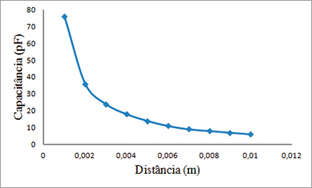
\includegraphics{img/cidepe-cxd.jpg}
	\caption{$C \times d$. Fonte: Cidepe.}
	\label{fig:imagem1}
\end{figure}

\begin{figure}[H]
	\centering
	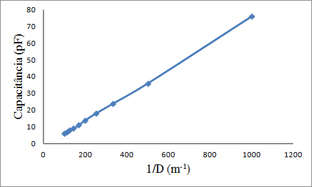
\includegraphics{img/cidepe-cx1d.jpg}
	\caption{$C \times 1/d$. Fonte: Cidepe.}
	\label{fig:imagem1}
\end{figure}

\textbf{Dicas}[B]

A capacitância é a principal propriedade de um capacitor, e diz respeito à capacidade de armazenamento das cargas elétricas. Podemos definir Capacitância como sendo a relação entre a quantidade de cargas acumuladas e a diferença de potencial aplicada às armaduras em um capacitor. Quanto maior a capacitância, maior a quantidade de cargas elétricas que podem ser armazenadas no dispositivo.


A capacitância é medida em uma unidade denominada Farad (batizada em homenagem ao célebre físico e químico Michael Faraday), abreviada pela letra F, e no geral os capacitores utilizam submúltiplos dessa unidade, pois a capacitância de 1 F é um valor muito elevado. Um capacitor de 1F conectado a uma fonte que forneça 1V de tensão elétrica irá armazenar uma carga de 1C, que equivale a 6,24 x 1018 elétrons.

As principais unidades utilizadas para representar a capacitância de um capacitor são as seguintes:

	%tabela 5
	\begin{table}[H]
		\centering
	\begin{tabular}{l|c|c}
		\hline 
		Nome da Unidade & Símbolo & Valor equivalente em Farads\\ 
		\hline 
		Milifarad & $m F$ & $1 \times 10^{-3}\,F$ \\ 
		Microfarad & $\mu F$ & $1 \times 10^{-6}\,F$ \\  
		Nanofarad & $n F$ & $1 \times 10^{-9}\,F$ \\  
		Picofarad & $p F$ & $1 \times 10^{-12}\,F$ \\ 
		\hline 
	\end{tabular} 
		\caption{Principais unidades de Capacitância}
		\label{tab:capacitancias}
	\end{table}

Um capacitor possui capacitância de um Farad quando uma carga elétrica de um Coulomb é armazenada em suas armaduras por uma tensão elétrica de um Volt. A capacitância é sempre um valor positivo.

\bibliographystyle{plain}
  \begin{thebibliography}{1}
    \bibitem{item-1} INSTITUTO DE FÍSICA GLEB WATAGHIN. “Aula 5: Capacitância”. Disponível em
<http://midia.cmais.com.br/assets/file/original/bc19adc4984d1dd3d06412d78fe66d166e7c3514.
pdf/>. Acesso em 12 de Julho de 2018.
    \bibitem{item-2} REDAÇÃO. “Resumo de física: Capacitância e tensão elétrica”. Disponível em
<https://guiadoestudante.abril.com.br/estudo/resumo-de-fisica-capacitancia-e-tensao-
eletrica/>. Acesso em 12 de Julho de 2018.
    \bibitem{item-3} BOSONTREINAMENTOS. "Treinamentos em Ciência e Tecnologia". Disponível em <http://www.bosontreinamentos.com.br/eletronica/curso-de-eletronica/especificacoes-dos-capacitores/>. Acesso em 25 de outubro de 2020.
    \bibitem{item-4} PLATO. "Ruptura Dielétrica". <http://plato.if.usp.br/~fge0211n/Main_Site/Extras/Extras_files/Ruptura%20diele%CC%81trica.pdf>. Acesso em 25 de outubro de 2020.
  \end{thebibliography}